\subsection{x86}

\subsubsection{MSVC}

Что получаем на ассемблере, компилируя в MSVC 2010:

\lstinputlisting{patterns/04_scanf/1_simple/ex1_MSVC_RU.asm}

Переменная \TT{x} является локальной.

По стандарту \CCpp она доступна только из этой же функции и нигде более. 
Так получилось, что локальные переменные располагаются в стеке. 
Может быть, можно было бы использовать и другие варианты, но в x86 это традиционно так.

\myindex{x86!\Instructions!PUSH}
Следующая после пролога инструкция \TT{PUSH ECX} не ставит своей целью сохранить 
значение регистра \ECX. 
(Заметьте отсутствие соответствующей инструкции \TT{POP ECX} в конце функции).

Она на самом деле выделяет в стеке 4 байта для хранения \TT{x} в будущем.

\label{stack_frame}
\myindex{\Stack!Стековый фрейм}
\myindex{x86!\Registers!EBP}
Доступ к \TT{x} будет осуществляться при помощи объявленного макроса \TT{\_x\$} (он равен -4) и регистра \EBP указывающего на текущий фрейм.

Во всё время исполнения функции \EBP указывает на текущий \glslink{stack frame}{фрейм} и через \TT{EBP+смещение}
можно получить доступ как к локальным переменным функции, так и аргументам функции.

\myindex{x86!\Registers!ESP}
Можно было бы использовать \ESP, но он во время исполнения функции часто меняется, а это не удобно. 
Так что можно сказать, что \EBP это \IT{замороженное состояние} \ESP на момент начала исполнения функции.

% FIXME1 это уже было в 02_stack?
Разметка типичного стекового \glslink{stack frame}{фрейма} в 32-битной среде:

\begin{center}
\begin{tabular}{ | l | l | }
\hline
\dots & \dots \\
\hline
EBP-8 & локальная переменная \#2, \MarkedInIDAAs{} \TT{var\_8} \\
\hline
EBP-4 & локальная переменная \#1, \MarkedInIDAAs{} \TT{var\_4} \\
\hline
EBP & сохраненное значение \EBP \\
\hline
EBP+4 & адрес возврата \\
\hline
EBP+8 & \argument \#1, \MarkedInIDAAs{} \TT{arg\_0} \\
\hline
EBP+0xC & \argument \#2, \MarkedInIDAAs{} \TT{arg\_4} \\
\hline
EBP+0x10 & \argument \#3, \MarkedInIDAAs{} \TT{arg\_8} \\
\hline
\dots & \dots \\
\hline
\end{tabular}
\end{center}

У функции \scanf в нашем примере два аргумента.

Первый~--- указатель на строку, содержащую \TT{\%d} и второй~--- адрес переменной \TT{x}.

\myindex{x86!\Instructions!LEA}
Вначале адрес \TT{x} помещается в регистр \EAX при помощи инструкции \TT{lea eax, DWORD PTR \_x\$[ebp]}.

Инструкция \LEA означает \IT{load effective address}, и часто используется для формирования адреса чего-либо ~(\myref{sec:LEA}).

Можно сказать, что в данном случае \LEA просто помещает в \EAX результат суммы значения в регистре \EBP и макроса \TT{\_x\$}.

Это тоже что и \INS{lea eax, [ebp-4]}.

Итак, от значения \EBP отнимается 4 и помещается в \EAX.
Далее значение \EAX заталкивается в стек и вызывается \scanf.

После этого вызывается \printf. Первый аргумент вызова строка:
\TT{You entered \%d...\textbackslash{}n}.

Второй аргумент: \INS{mov ecx, [ebp-4]}.
Эта инструкция помещает в \ECX не адрес переменной \TT{x}, а её значение.

Далее значение \ECX заталкивается в стек и вызывается \printf.

\clearpage
\subsection{MSVC + \olly}
\index{\olly}

\RU{Попробуем этот же пример в}\EN{Let's try this example in} \olly.
\RU{Загружаем, нажимаем F8 (\stepover) до тех пор, пока не окажемся в своем исполняемом файле,
а не в}\EN{Let's load it and keep pressing F8 (\stepover) until we reach our executable file
instead of} \TT{ntdll.dll}.
\RU{Прокручиваем вверх до тех пор, пока не найдем \main}\EN{Scroll up until \main appears}.
\RU{Щелкаем на первой инструкции (\TT{PUSH EBP}), нажимаем F2 (\IT{set a breakpoint}), 
затем F9 (\IT{Run}) и точка останова срабатывает на начале \main.}
\EN{Click on the first instruction (\TT{PUSH EBP}), press F2 (\IT{set a breakpoint}), 
then F9 (\IT{Run}).
The breakpoint will be triggered when \main begins.}

\RU{Трассируем до того места, где готовится адрес переменной $x$}%
\EN{Let's trace to the point where the address of the variable $x$ is calculated}:

\begin{figure}[H]
\centering
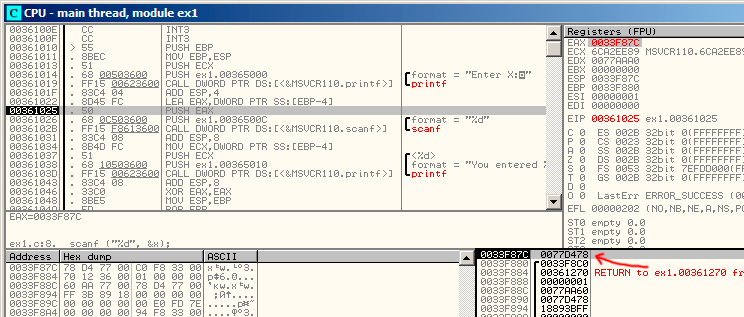
\includegraphics[scale=\FigScale]{patterns/04_scanf/1_simple/ex1_olly_1.png}
\caption{\olly: \RU{вычисляется адрес локальной переменной}\EN{The address of the local variable is calculated}}
\label{fig:scanf_ex1_olly_1}
\end{figure}

\RU{На \EAX в окне регистров можно нажать правой кнопкой и далее выбрать}
\EN{Right-click the \EAX in the registers window and then select} \q{Follow in stack}.
\RU{Этот адрес покажется в окне стека.}
\EN{This address will appear in the stack window.}
\RU{Смотрите, это переменная в локальном стеке. Я нарисовал там красную стрелку}\EN{The red arrow, I have added, points to the variable in the local stack}.
\RU{И там сейчас какой-то мусор}\EN{At that moment this location contains some garbage} (\TT{0x6E494714}).
\RU{Адрес этого элемента стека сейчас, при помощи \PUSH запишется в этот же стек рядом}%
\EN{Now with the help of \PUSH instruction the address of this stack element is going to be stored to the same stack on the next position}.
\RU{Трассируем при помощи F8 вплоть до конца исполнения \scanf}\EN{Let's trace with F8 until the \scanf execution completes}.
\RU{А пока \scanf исполняется, в консольном окне, вводим, например, 123}%
\EN{During the \scanf execution, we input, for example, 123, in the console window}:

\begin{figure}[H]
\centering
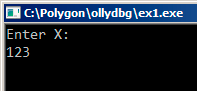
\includegraphics[scale=\NormalScale]{patterns/04_scanf/1_simple/ex1_olly_2.png}
\caption{\RU{Ввод пользователя в консольном окне}\EN{User input in the console window}}
\label{fig:scanf_ex1_olly_2}
\end{figure}

\clearpage
\RU{Вот тут }\scanf \RU{отработал}\EN{completed its execution already}:

\begin{figure}[H]
\centering
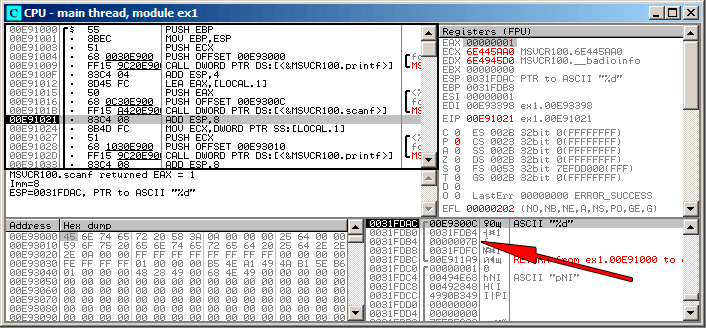
\includegraphics[scale=\FigScale]{patterns/04_scanf/1_simple/ex1_olly_3.png}
\caption{\olly: \scanf \RU{исполнилась}\EN{executed}}
\label{fig:scanf_ex1_olly_3}
\end{figure}

\scanf \RU{вернул}\EN{returns} $1$ \InENRU \EAX, \RU{что означает, что он успешно прочитал одно 
значение}\EN{which implies that it has read successfully one value}.
\RU{В наблюдаемом нами элементе стека теперь}\EN{If we look again at the stack element corresponding to the local variable it now contains} \TT{0x7B} (123).

\clearpage
\RU{Чуть позже это значение копируется из стека в регистр \ECX и передается в \printf}
\EN{Later this value is copied from the stack to the \ECX register and passed to \printf}:

\begin{figure}[H]
\centering
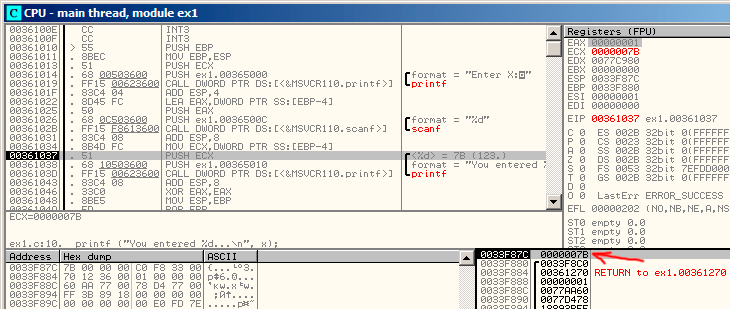
\includegraphics[scale=\FigScale]{patterns/04_scanf/1_simple/ex1_olly_4.png}
\caption{\olly: \RU{готовим значение для передачи в}\EN{preparing the value for passing to} \printf}
\label{fig:scanf_ex1_olly_4}
\end{figure}


\subsubsection{GCC}

Попробуем тоже самое скомпилировать в Linux при помощи GCC 4.4.1:

\lstinputlisting{patterns/04_scanf/1_simple/ex1_GCC.asm}

\myindex{puts() вместо printf()}
GCC заменил первый вызов \printf на \puts. Почему это было сделано, 
уже было описано ранее~(\myref{puts}).

% TODO: rewrite
%\RU{Почему \scanf переименовали в \TT{\_\_\_isoc99\_scanf}, я честно говоря, пока не знаю.}
%\EN{Why \scanf is renamed to \TT{\_\_\_isoc99\_scanf}, I do not know yet.}
% 
% Apparently it has to do with the ISO c99 standard compliance. By default GCC allows specifying a standard to adhere to.
% For example if you compile with -std=c89 the outputted assmebly file will contain scanf and not __isoc99__scanf. I guess current GCC version adhares to c99 by default.
% According to my understanding the two implementations differ in the set of suported modifyers (See printf man page)


Далее всё как и прежде~--- параметры заталкиваются через стек при помощи \MOV.

\subsubsection{Кстати}

Кстати, этот простой пример иллюстрирует то обстоятельство, что компилятор преобразует
список выражений в \CCpp-блоке просто в последовательный набор инструкций.
Между выражениями в \CCpp ничего нет, и в итоговом машинном коде между ними тоже ничего нет, 
управление переходит от одной инструкции к следующей за ней.

